\documentclass{article}

\usepackage[a4paper, margin=2cm]{geometry}
\usepackage[utf8]{inputenc}

\usepackage[czech]{babel}
\usepackage{fvextra}
\usepackage{csquotes}
\usepackage{parskip}
\usepackage{expl3}

\usepackage{float}
\usepackage{amsmath}
\usepackage{textcomp}
\usepackage{gensymb}
\usepackage{graphicx}
\graphicspath{{images}}

\usepackage[style=verbose-ibid]{biblatex}
\addbibresource{refs.bib}

\usepackage[hidelinks, unicode, pdfusetitle]{hyperref}

\usepackage{mathtools}
\DeclarePairedDelimiter\ceil{\lceil}{\rceil}
\DeclarePairedDelimiter\floor{\lfloor}{\rfloor}

\title{34-3-X1 Dráteníci}
\author{Benjamin Swart}

\setcounter{secnumdepth}{1}

\begin{document}

\maketitle

\section{Algoritmus pro natažení kabelů}
\label{section:base}

Nejprve napíšeme algoritmus, který předpokládá, že máme počet barev daný a stačí nám jen určit, kudy jaké kabely povedou.

\begin{figure}[H]
    \centering
    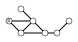
\includegraphics[scale=0.7]{initial.pdf}
\end{figure}

Můžeme využít algoritmus pro tok v síti. Aby se nám barvy nepomíchaly, tak vytvoříme kopii sítě pro každou barvu kabelu. Protože každou trubkou smí vést každá barva jen jednou, tak bude kapacita všech hran 1. Routery nahradíme zdrojem. Hrany jsou (zatím) obousměrné.

\begin{figure}[H]
    \centering
    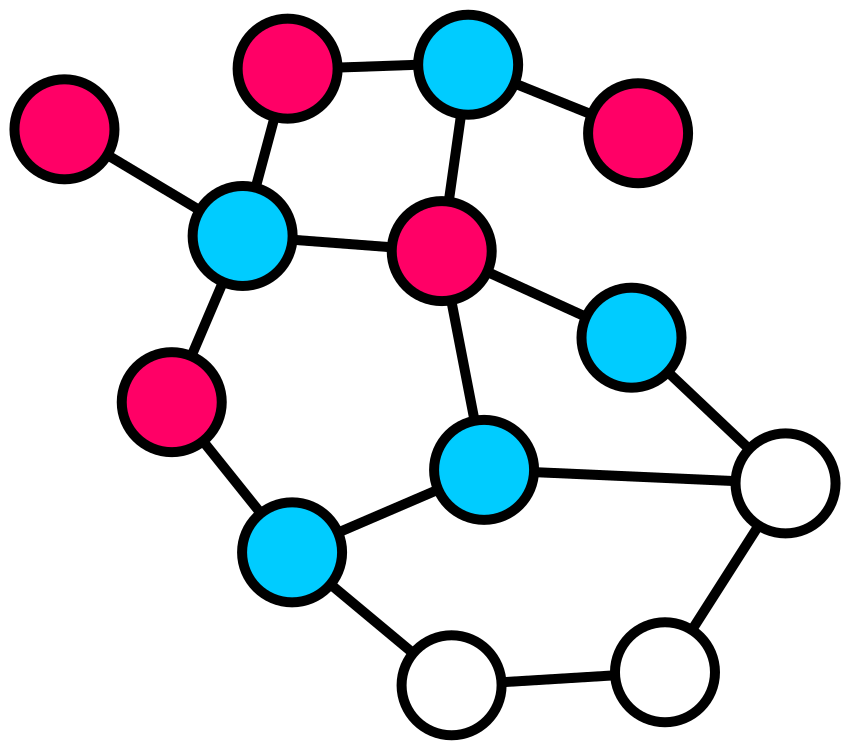
\includegraphics[scale=0.7]{colored.pdf}
\end{figure}

Nakonec musíme nějak reprezentovat stoky. V každém z původích vcholů potřebujeme ukončit právě jeden kabel. Pro každý vrchol vytvoříme vrchol nový, do kterého orientovanou hranou\footnote{Kapacita těchto hran je jedna, ale mohla by být i větší.} připojíme všechny jeho barevné varianty. Nakonec tento vrchol spojíme hranou s kapacitou 1 se stokem.

\begin{figure}[H]
    \centering
    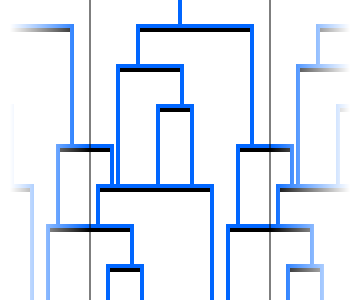
\includegraphics[scale=0.7]{full.pdf}
\end{figure}

Tím docílíme toho, že můžeme v každém vrcholu ukončit právě jednu barvu kabelu (a právě jeden kabel od té barvy).

Následně musíme spojit zdroje a stoky a změnit neorientované hrany v orientované jak je popsáno v kuchařce. Poté spustíme algoritmus na nalezení maximálního průtoku sítě. Kuchařka uvádí Fordův-Fulkersonův algoritmus, který běží v čase \(O(nm^2)\).\footnote{Kde \(n\) je počet vrcholů a \(m\) je počet hran.} Na internetu se můžeme dočíst o článku\footcite{max-flow-onm}, který popisuje algoritmus v \(O(nm)\), ačkoliv se přiznám, že jsem ho nečetl. Složitost algoritmu pro tok v síti s \(n\) vrcholy a \(m\) hranami označím \(F(n, m)\). Zajímavé je, že v mém grafu mají všechy hrany ohodnocení buď \(1\) nebo \(\infty\), čehož by se možná dalo využít.

Z grafu ohodnoceného průtokem není těžké zrekonstruovat kabely. Zaprvé se můžeme podívat, jestli je průtok rovný počtu domů. Pokud tomu tak není, tak je úhloha pro daný počet barev neřešitelná. Pokud tomu tak je, tak stačí z routeru vyjít nějakou trubkou s průtokem 1, tento průtok smazat, a takto dále hladově plnit trubky, dokud neskončíme ve stoku nějakého domu, kde kabel zakončíme. Toto opakujeme, dokud máme, jak se z routeru dostat. Je sice možné, že po cestě vytvoříme zbytečné kličky, ale to nevadí. Do každého domu nějaký kabel nutně zavedeme.

\begin{figure}[H]
    \centering
    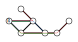
\includegraphics[scale=0.7]{wired.pdf}
\end{figure}

Časová složitost tohoto algoritmu bude \(O(F(nc, mc))\), kde \(c\) je počet barev. Jelikož všechny průtoky, které tahání kabelů projde, musel algoritmus pro tok v síti vypočítat, je vyloučeno, že by bylo tahání kabelů nejpomalejším krokem v našem algoritmu.

\section{Hledání počtu barev}

Počet barev můžeme najít exponenciálním vyhledáváním. Spustíme algoritmus z sekce \ref{section:base} s počtem barev 1. Pokud nenajde řešení, tak ho spustíme znovu s počtem 2. Pokud to nebude stačit, tak zkusíme 4, pokud to nepůjde, tak 8 atd. Jakmile najdeme nějaký počet barev \(b\), který bude stačit, tak přesný hraniční počet barev najdeme klasickým binárním vyhledáváním mezi \(b/2\) a \(b\).

Exponenciální vyhledávání použije \(O(log(c))\) dotazů, kde \(c\) je nalezený minimální počet barev. Každý dotaz zabere maximálně \(O(F(nc, mc))\) času, takže celková časová složitost algoritmu bude \(O(F(nc, mc)*log(c))\). Pokud použijeme algoritmus z kuchařky, tak bude složitost \(O(nm^2c^2*log(c))\).

Paměťová složitost bude \(O(nc+mc)\).

Nejdená se o příliž rychlý algoritmus, ale alespoň je polynomiální.

\end{document}
